\subsubsection{Esquema de despliegue tecnológico}

El sistema y el agente conversacional comparten una única infraestructura.

\paragraph{Diagrama de despliegue}

La Figura~\ref{fig:ob2_despliegue} muestra los nodos del despliegue y cómo se comunican. Los servicios se empaquetan como contenedores \cite{docker2024containers}, y la Tabla~\ref{tab:ob2_nodos} resume la función de cada nodo.

\begin{figure}[H]
\centering
\IfFileExists{diagramas/drawio/Despliegue.png}{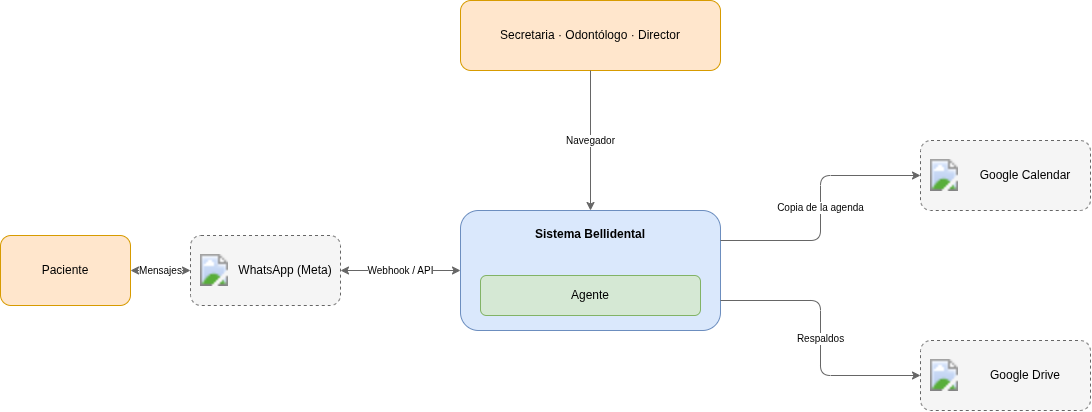
\includegraphics[width=\linewidth]{diagramas/drawio/Despliegue.png}}{\fbox{\parbox{0.9\linewidth}{\centering Pendiente: dibujar según diagramas/drawio/ESPECIFICACION-despliegue.md y exportar a img/Despliegue.pdf}}}
\caption{Diagrama de despliegue del sistema y del agente (UML)}
\label{fig:ob2_despliegue}
\end{figure}

\begin{table}[H]
\centering
\caption{Nodos del diagrama de despliegue}
\label{tab:ob2_nodos}
\fontsize{9}{11}\selectfont
\renewcommand{\arraystretch}{1.2}
\setlength{\tabcolsep}{4pt}
\begin{tabularx}{\linewidth}{|>{\raggedright\arraybackslash}p{4.0cm}|>{\raggedright\arraybackslash}X|}
\hline
\textbf{Nodo} & \textbf{Función} \\ \hline
Equipos de la clínica & Usan la aplicación web desde el navegador, sin instalación \\ \hline
Teléfono del paciente & Conversa con el agente y recibe recordatorios por WhatsApp \\ \hline
Servidor virtual (VPS) & Ejecuta con Docker Compose el proxy nginx, la API con el agente, PostgreSQL y el respaldo \\ \hline
WhatsApp Cloud API (Meta) & Entrega los mensajes al webhook y envía las respuestas \\ \hline
Google Calendar & Recibe la copia de la agenda \\ \hline
Google Drive de la clínica & Guarda los respaldos cifrados fuera del servidor \\ \hline
\end{tabularx}
\end{table}

El agente solo añade a esta infraestructura el webhook por HTTPS \cite{meta2026whatsapp}, un número de WhatsApp registrado en la Cloud API y las plantillas de mensaje aprobadas por Meta.

\paragraph{Entornos}

El despliegue se organiza en dos entornos (Tabla~\ref{tab:ob2_entornos}). Ambos operan en el modo de producción básico de la Cloud API, que permite usar un número telefónico real sin la verificación de la empresa ante Meta. El desarrollo usa el número del desarrollador; la producción, el número de la recepción.

\begin{table}[H]
\centering
\caption{Entornos de despliegue}
\label{tab:ob2_entornos}
\fontsize{9}{11}\selectfont
\renewcommand{\arraystretch}{1.2}
\setlength{\tabcolsep}{4pt}
\begin{tabularx}{\linewidth}{|>{\raggedright\arraybackslash}p{2.4cm}|>{\raggedright\arraybackslash}p{4.0cm}|>{\raggedright\arraybackslash}p{4.0cm}|>{\raggedright\arraybackslash}X|}
\hline
\textbf{Entorno} & \textbf{WhatsApp} & \textbf{Infraestructura} & \textbf{Datos} \\ \hline
Desarrollo & Número real del desarrollador, en modo básico sin verificación de la empresa & Equipo local con Docker Compose y un túnel (ngrok) para el webhook & Ficticios \\ \hline
Producción & Número de la recepción, en modo básico sin verificación de la empresa & VPS contratado a nombre de la clínica & Reales de la clínica \\ \hline
\end{tabularx}
\end{table}

El paso de desarrollo a producción solo cambia el número configurado y exige aprobar las plantillas en la cuenta de la clínica; el diseño no cambia. El modo básico mantiene el límite inicial de envío de mensajes iniciados por la empresa, suficiente para los recordatorios diarios de la clínica. La verificación de la empresa ante Meta, que eleva ese límite, no forma parte del alcance y se plantea como recomendación.

\paragraph{Riesgos y mitigaciones}

La Tabla~\ref{tab:ob2_riesgos} identifica los riesgos del despliegue en un servidor virtual, sus efectos y sus mitigaciones.

\begingroup
\fontsize{9}{11}\selectfont
\renewcommand{\arraystretch}{1.2}
\setlength{\LTpre}{0pt}\setlength{\LTpost}{6pt}
\setlength{\tabcolsep}{4pt}
\begin{longtable}{|p{0.26\linewidth}|p{0.28\linewidth}|p{0.36\linewidth}|}
\caption{Riesgos del despliegue y mitigaciones}
\label{tab:ob2_riesgos} \\
\hline
\textbf{Riesgo} & \textbf{Efecto} & \textbf{Mitigación} \\ \hline
\endfirsthead
\hline
\textbf{Riesgo} & \textbf{Efecto} & \textbf{Mitigación} \\ \hline
\endhead
\hline
\endfoot
Impago o cierre del VPS & Caída total del sistema y del agente & Cuenta a nombre de la clínica; respaldo y exportación para migrar \\ \hline
Caída de internet en la clínica & Personal sin acceso; el agente sigue activo & Ficha en papel y carga posterior \\ \hline
Pérdida del servidor & Hasta 24 h de datos perdidos & Restauración desde el respaldo diario externo \\ \hline
Datos tratados fuera del Ecuador & Datos personales fuera del control de la clínica & Contrato de encargado (LOPDP \cite{lopdp2021}); respaldos cifrados; Meta y Google solo reciben datos de la cita \\ \hline
Suspensión de la cuenta de WhatsApp & Sin agente ni recordatorios & Plantillas aprobadas; recepción como canal alterno \\ \hline
Agotamiento de recursos & Lentitud o caída de contenedores & Límite de memoria por contenedor (0,6 a 1 GB estimados) \\ \hline
\end{longtable}
\endgroup

\textbf{Cambio frente a la instalación local prevista inicialmente.} En la Entrevista 1 (Tabla~\ref{tab:ent1}, P7), el Director pidió que la continuidad y la propiedad de la información no dependieran de un proveedor externo; de ahí deriva RNF04. El VPS reintroduce esa dependencia, que se mitiga con cuatro medidas: la cuenta del VPS y el dominio a nombre de la clínica, el respaldo diario bajo la cuenta de la clínica, la exportación completa en formato abierto y el mismo archivo de Docker Compose, que permite migrar a otro proveedor o a la instalación local. A cambio, el VPS mantiene el agente disponible fuera del horario sin depender de un equipo encendido en la clínica. La disponibilidad del sistema en horario de atención (RNF05) queda sujeta a la conexión de la clínica; durante una caída, la ficha rápida en papel y la carga posterior sostienen la atención.

\paragraph{Alternativa de instalación local}

Si la clínica no contrata un servidor virtual, el sistema se instala en el equipo de recepción. Ese equipo cumple el rol del VPS, y el mismo archivo de Docker Compose sirve a ambas modalidades. La Tabla~\ref{tab:ob2_local} resume las diferencias.

\begin{table}[H]
\centering
\caption{Diferencias entre el servidor virtual y la instalación local}
\label{tab:ob2_local}
\fontsize{9}{11}\selectfont
\renewcommand{\arraystretch}{1.2}
\setlength{\tabcolsep}{4pt}
\begin{tabularx}{\linewidth}{|>{\raggedright\arraybackslash}p{3.0cm}|>{\raggedright\arraybackslash}p{4.6cm}|>{\raggedright\arraybackslash}X|}
\hline
\textbf{Elemento} & \textbf{Servidor virtual (VPS)} & \textbf{Instalación local} \\ \hline
Servidor & VPS contratado a nombre de la clínica & Equipo de recepción, encendido de forma permanente \\ \hline
Webhook & Proxy inverso nginx con Let's Encrypt & Túnel de Cloudflare que expone solo el webhook \\ \hline
Respaldos & Volcado diario en Google Drive de la clínica & Volcado diario en un disco externo, separado del equipo \\ \hline
Disponibilidad & Continua, sujeta al proveedor y, para el personal, a la conexión de la clínica & Limitada al encendido del equipo; el agente no responde con el equipo apagado \\ \hline
Uso sin internet & No & Sí, para la recepción y los consultorios en la red local \\ \hline
\end{tabularx}
\end{table}
